\chapter{Scientific Background}
%labels will help you to reference to certain images, tables, chapters, section, and so on...
\label{background}

% DELETEME: This chapter will cover all of your background information and related work. Background and related work are directly related to your thesis. Please do not place irrelevant content here which is a common mistake. Citing will be handled in the appendices.

% DELETEME: Background represents underlying knowledge that is required to understand your work. The expected knowledge level of your readers can be set to the one of a bachelor or master student who just finished his studies (depending on what kind of thesis you are writing). This means that you do not need to describe how computers work, unless your thesis topic is about this. Everything that an average alumnus from your field of studies should know does not need to be described. It turns, background information that is very complex and content-wise very near to your problem, can be placed in the main parts. Everything else should be written here. Note: it is important to connect each presented topic to your thesis. E.g. if you present the ISO/OSI layer model you should also write that this is needed to understand the protocols you plan to develop in the main parts.

% DELETEME: Related work represents results from work that handled the same or a similar problem that you are addressing. This work might have used a different approach or might not have been that successful. Finding a paper / work that solved your problem in the same way you were planning to do is not good and you should contact your supervisor for solving this issue. Again, each paper / work has to be connected to your approach: other papers might have not chosen an optimal solution; they might not have been taking care of essential aspects; they might have chosen a different approach and you believe, yours will work better ...

This chapter introduces some important scientific fundamentals for better understanding of the problem's solution. Initially, \ref{camera_section} explains about the composition of a single digital pinhole camera and some of its characteristics. Then, \ref{camera_model} outlines the mathematical model for transforming a 3D object on the 2D image plane. In section \ref{carla_background} it is described how the 3D autonomous driving simulator works, its design is explained and some important CARLA's terms used in this work are presented. Afterwards, the subsection \ref{instance_camera} informs about the functionality of the RGB and the instance segmentation camera that CARLA offers. Finally, we talk about the related work in section \ref{related_work}.

%###################################################################################
%###################### Topic A             ########################################
%###################################################################################
\section{Camera}\label{camera_section}
The digital camera is an instrument used for creating images through capturing light and converting it into colourful pixels. On the Figure \ref{fig:camera_construction} we could get an idea of how this technological invention is constructed. It uses an optic that consists of one or more lenses, through which the light rays are received. Afterwards, there is a sensor resembling the form of a solar panel, divided into red, green and blue pixels, which is hit by the collected light rays. As described from Schreer in \cite{camera_pinhole_model} the process of transforming the information from the captured light into a meaningful for the human eye representation is the following one: 
\begin{itemize}
    \item Light ray hits a sensor's pixel $\rightarrow$ The sensor converts it into an energy signal, which sends to the built-in computer $\rightarrow$ The computer estimates how dark or light the according pixel on the image plane should be and determines the correct colour value $\rightarrow$ As an output all pixels are combined in order to approximately recreate all details from the captured object  
\end{itemize}

\begin{figure}[h]
\centering
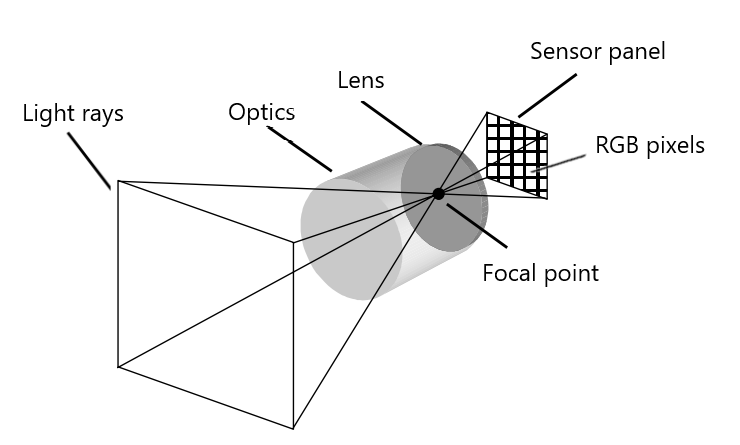
\includegraphics[width=0.8\textwidth]{images/camera_construction.png}
\caption[Digital camera's design]{This image illustrates simply the design of a digital camera, from Schreer's book \cite{camera_pinhole_model} (Fig. 3.1) with some changes. Labels were translated to English and some new ones were added. \label{fig:camera_construction}}
\end{figure}

\newpage
In order to display a more detailed version of the captured image, cameras need more pixels to collect light rays\footnote{\url{https://www.creativelive.com/photography-guides/how-does-a-camera-work}, visited on 18/11/2022}. Thus, modern cameras rely on a bigger number of pixels to enhance the quality of the photos, which also contributes to improving the resolution of the visual sensor. Cameras with greater resolution are important in the area of street surveillance because in case of accidents or an against-the-rules behaviour it facilitates the task of recognising the suspect. Moreover, when we take into account the fact that these sensors act as a visual world perception for the autonomous vehicles, the resolution plays an essential role in the efficient object detection \cite{resolution_importance}. 

Another specification of cameras that this thesis considers is the so-called field of view (FoV), which determines the quantity of information that has been captured on the result image. It depends on the focal length of the lens and the sensor's size. On Figure \ref{fig:camera_fov} is shown what happens when the light goes through the lenses. In the upper case, due to a shorter focal length\footnote{The length between the lens and the focused image on the sensor} the lens converges the light stronger, therefore the focus is on the subject being imaged and the FoV is larger. In the vice-versa situation, the longer focal length allows for a focus on the image and thus provides a smaller FoV.

The monocular cameras belong to the directional sensors, because they can perceive information only from the direction in which their optical part is adjusted. In contrast to LiDAR sensors, which has a 360$^{\circ}$ view of the environment around it and can not be affected by light
conditions, single cameras are unreliable when exposed to bad light and weather conditions \cite{camera_vs_lidar}. As a main drawback of single cameras is regarded the lack of depth information, which impedes an accurate object recognition. Nevertheless, monocular cameras have advantages like lower integration price, much bigger availability on the market and the most important one is that they provide detailed pixel intensity information in form of a visual representation of the real world.

\begin{figure}[h]
\centering
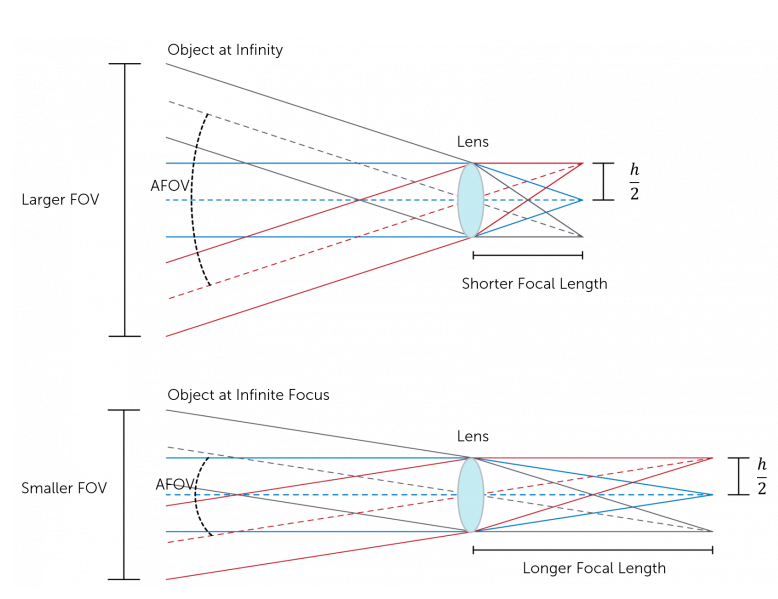
\includegraphics[width=0.8\textwidth]{images/camera_fov.png}
\caption[Single camera's FoV]{Depicting the influence of the focal length on the field of view, authored by \cite{camera_fov_website} \label{fig:camera_fov}}
\end{figure}

\subsection{Camera model}\label{camera_model}
In order to illustrate how the transformation from a 3D world coordinate point to a 2D sensor's coordinate system happens, we use the pinhole camera model from Schreer \cite{camera_pinhole_model}. Figure \ref{fig:camera_model} portrays how a point $M(X_{w}, Y_{w}, Z_{w})^{T}$ from a real world's object placed in front of the camera is orthogonally projected on the image plane. We define the projected point $m$ in the image plane's coordinate system as $m(u,v)^{T}$. As we can see, the projection center stays behind the image plane and its optical axis points in the Z-direction, therefore it intersects the image plane in the principle point $c$. When we want to define the location of a 3D world point on the image plane we have to use the camera's intrinsic matrix $A$, which contains parameters of the camera like the coordinates of the principle point $c(u_{0},v_{0})$, the scale factors $\alpha$ and $\beta$ of the $u$ and $v$ image axes and their skew index denoted by $\gamma$, which is 0 in ideal conditions with no distortion. We get $\alpha$ and $\beta$ by dividing the focal length $f$ and the pixel size $\delta$ . In the following equation we execute a matrix multiplication between the intrinsic matrix $A$ and a normalized 3x4 matrix $P_{N}$:

\begin{equation}
    P_{new} = A P_{N} = \begin{bmatrix}
                        \alpha & \gamma & u_{0}\\
                        0 & \beta & v_{0}\\
                        0 & 0 & 1\end{bmatrix} \cdot \begin{bmatrix}
                        1 & 0 & 0 & 0\\
                        0 & 1 & 0 & 0\\
                        0 & 0 & 1 & 0\end{bmatrix} \: , where \: \alpha, \beta = f / \delta
\end{equation}

As an output of the equation we receive the projection matrix $P_{new}$ and the last step is to transform the world coordinates of the point $M$ into the sensor's coordinate system. We use a Euclidean homography matrix $H$, which contains the extrinsic parameters $(R,t)$ (rotation and translation) that create a relation between world coordinates and camera coordinates. Then we apply multiplication between $H$ and the point $M$ coordinates. The final step is to multiply the projection matrix with the result. The above-mentioned process is the following one:

\begin{equation}
m = P_{new} \cdot H \cdot M \:, with \: H = [R|t] 
\end{equation}

\begin{figure} [h!]
\centering
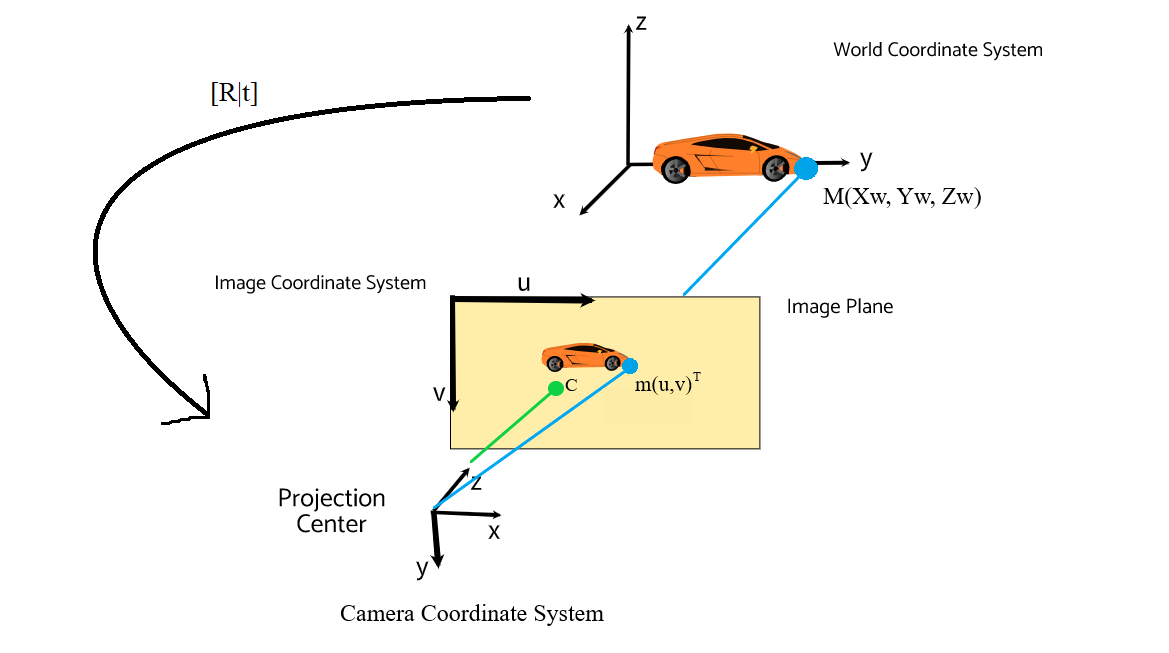
\includegraphics[width = \textwidth, height = 9cm]{images/camera_model_pic.png}
\caption[Single camera's model]{Schema of the pinhole model and a projection of a 3D object on a 2D image plane, based on \cite{camera_pinhole_model} (Fig. 3.5) and \cite{second_model_of_camera} (Fig. 1) \label{fig:camera_model}}
\end{figure}

%###################################################################################
%###################### Topic B             ########################################
%###################################################################################
\section{CARLA - 3D autonomous driving simulator}\label{carla_background}
In this section we introduce the open-source 3D simulator CARLA (Car Learning to Act) which runs as a layer over Unreal Engine 4 with the main purpose of facilitating autonomous driving research. The simulation platform provides a great number of open digital assets like buildings, vehicles, pedestrians, whole cities, etc. What is more, the simulator is constantly developed by a community of different developers, who contribute to a realistic digital environment and an efficient conducting of experiments and tests. In addition to the aforementioned benefits, CARLA gives the opportunity to researchers to work with urban layouts without having to consider any logistical difficulties of training and testing systems in the physical world or infrastructure costs \cite{carla_paper}. 

In contrast to the real world, inside the Unreal-Engine-based platform users are not limited to using a couple of vehicles, which enables them to cover a multitude of edge cases that are necessary for training and validation. Experiments often involve some kind of sensor, whose implementation and setup could be expensive and time-consuming, thus we use CARLA for this work, because it offers various types of sensors\footnote{\url{https://carla.readthedocs.io/en/latest/ref_sensors/}, visited on 20/11/2022} like RGB camera, depth camera, instance and semantic segmentation camera, LiDAR and radar systems.

CARLA is developed as a client-server application, where the client communicates with the server through sockets. The client API is programmed in Python, and realises an interaction with the server by sending user-implemented Python scripts in return for sensor data. Simultaneously, the server's task is to render the received client data in a running simulation. There are two types of commands that the client could send:
\begin{itemize}
    \item \textbf{normal commands} - control the world actors like vehicles or pedestrians and can modify all their attributes
    \item \textbf{meta-commands} - reset the simulation, define the server's behaviour, are responsible for the sensors and can apply different environmental settings like weather conditions or traffic density
\end{itemize}

Figure \ref{fig:carla_arch} presents a more detailed view about the scalable client-server architecture CARLA runs on. The server uses Unreal Engine 4 and Carla Plugins to create a realistic simulation of an urban environment, whereas the client communicates with it over TCP. This type of architecture allows multiple clients to connect with the server at the same time, although it is advisable to avoid it, because these are controlled by the developer and collisions could appear. It can be seen on the diagram that the CARLA API combines Python scripts and C++, which bring with itself the benefits of an uncomplicated environment for developers and a lower-lever robust communication. When the client is already connected to the server it can control the world actors and their behaviour as well. For instance, it uses a traffic manager to recreate a real-life traffic situations and define speed, direction, acceleration or other vehicle's attributes.

\begin{figure} [h]
\centering
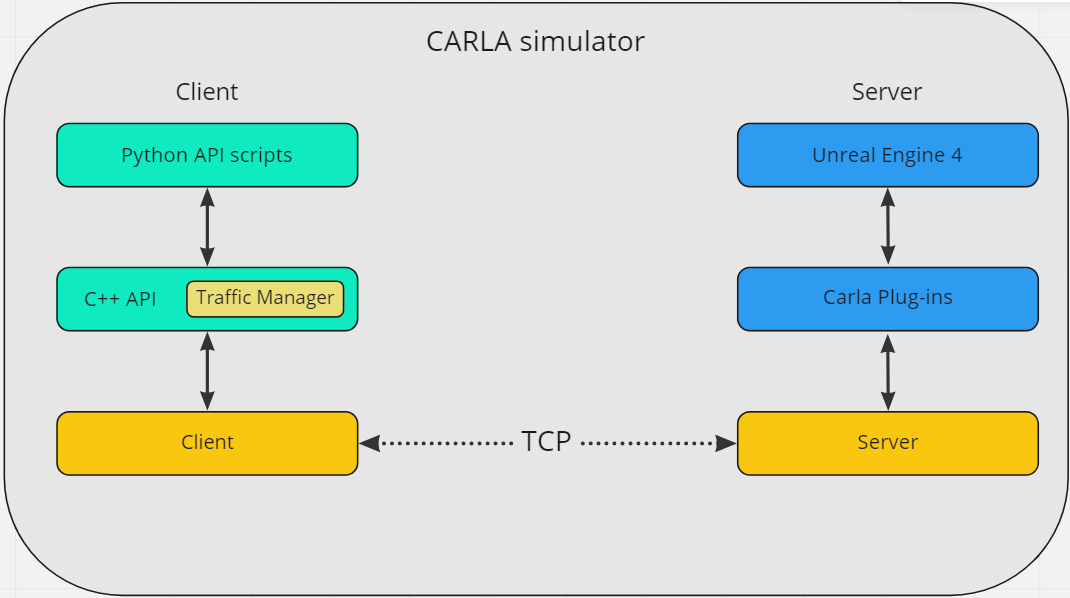
\includegraphics[width = 0.9\textwidth]{images/carla_arch.png}
\caption[CARLA's architecture]{Schema of CARLA's client-server architecture, based on \cite{carla_architecture} (Fig. 4) \label{fig:carla_arch}}
\end{figure}

After the in-depth explanation of CARLA's design, we introduce some terms and their definitions which are important for this work. In CARLA, objects like vehicles, sensors and pedestrians are called actors\footnote{\url{https://carla.readthedocs.io/en/latest/python_api/\#carlaactor}, visited on 20/11/2022}. A user can modify their location or rotation, which consists of pitch, yaw and roll (dimensions of movement through a medium), as well as other attributes of them. What is more, each actor has a ground truth bounding box\footnote{\url{https://carla.readthedocs.io/en/latest/python_api/\#carlaboundingbox}, visited on 20/11/2022}, that is a cuboid which contains the whole 3D object and could be used in object detection or tracking methods for example. 

In this work we mention the terms world and sensor/vehicle coordinates, because the coordinate system differs in regard to the point of view. When we place an actor in the simulator, then we use world coordinates for the location. In this way the server is constantly aware of their position and can inform the client in case of collisions. On the other side, an object's coordinate system begins from the center of its bounding box. Therefore, we always have to convert points into the same coordinate system in order to prevent unexpected errors.    

\subsection{RGB and Instance Segmentation Camera}\label{instance_camera}
In the above section we mentioned that CARLA supports different sensor types, among which the RGB and instance segmentation camera, which are the main focus of this thesis. The user defines a location in the simulator's world coordinates where a sensor should be spawn and apart from that the rotation of the sensor is adjusted to retrieve data from a specified direction. Furthermore, CARLA provides various basic and advanced camera attributes like FoV, image width, image height, lens distortion, calibration constant, etc\footnote{\url{https://carla.readthedocs.io/en/latest/ref_sensors/\#rgb-camera}, visited on 20/11/2022}. The output of the RGB camera is sensor-related information and raw data, which contains an array consisting of BGRA (blue, red, green and opacity index) 32-bit pixels.

For the purpose of a better differentiation between objects of the same type, CARLA implements the instance segmentation camera\footnote{\url{https://carla.readthedocs.io/en/latest/ref_sensors/\#instance-segmentation-camera}, visited on 20/11/2022}. Unlike the RGB camera, this one does not display the object's real colours. It classifies them by class and instance ID, during which a tag is assigned to every pixel on the image plane according to the type of object (vehicle, building, road, traffic sign, etc) it contains \cite{instance_segmenatation_cam}. In the output we receive again a BGRA array, but the pixels consist of the following colour values:
\begin{itemize}
    \item \textbf{Red channel} - contains a tag value from 0-22, for each type of object it belongs to. Apart from the pre-defined tags, the user can create new ones.
    \item \textbf{Green and Blue channel} - provide information about the internal ID of the object, which was set when it was initialised from Unreal Engine. We can retrieve the ID by solving this equation: $ID \: =  B + G * 256$, where G and B are the green and blue values respectively.
\end{itemize}

The information we get from an instance segmentation camera is useful for experiments, where we lack depth data and do not know whether one vehicle is located in front of another one. Moreover, the ground truth data contributes to more accurate and reliable results from the conducted experiments. To get an idea of the colour palette that the two cameras apply, we can have a look at the pictures below in Figure \ref{fig:camera_outputs}. 

\begin{figure} [h!]
  \centering
  \subfloat[RGB camera]{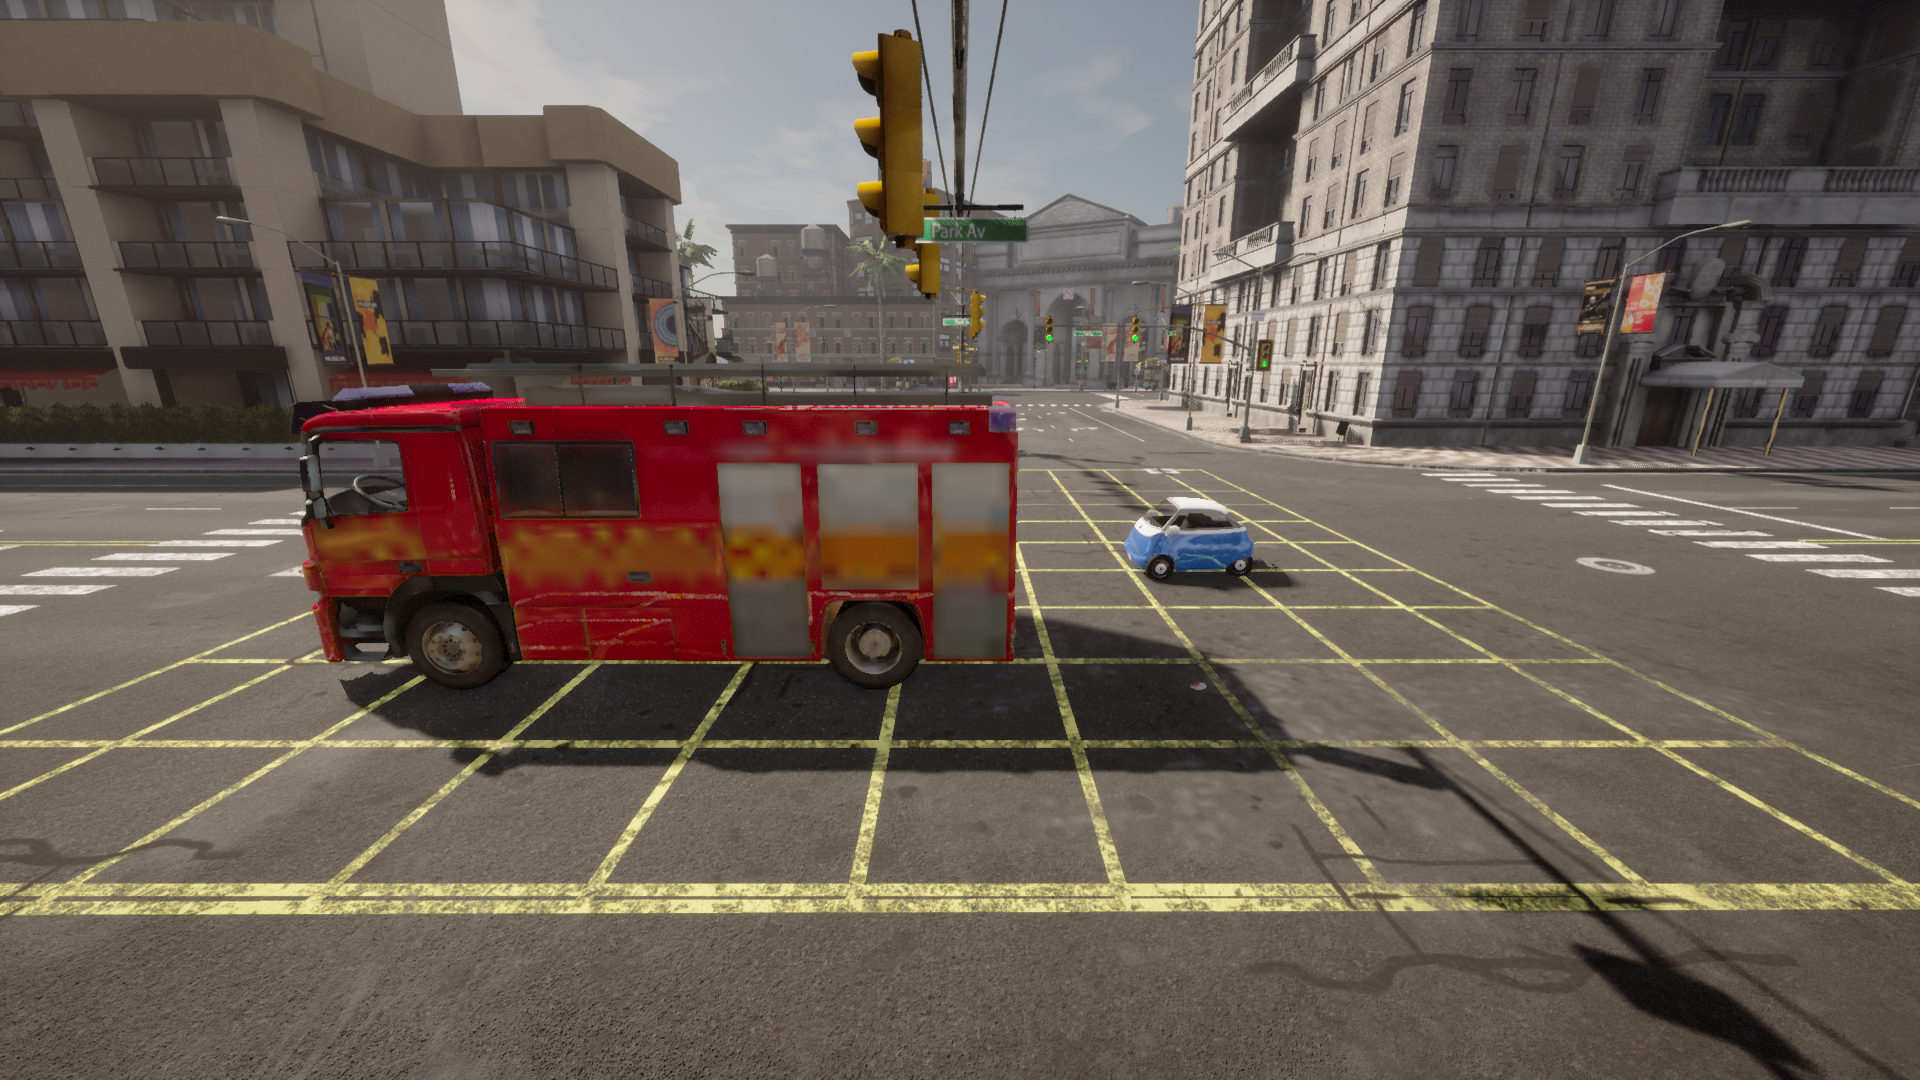
\includegraphics[width=0.5\textwidth]{images/rgb_cam.jpg}}
  \hfill
  \subfloat[Instance segmentation camera]{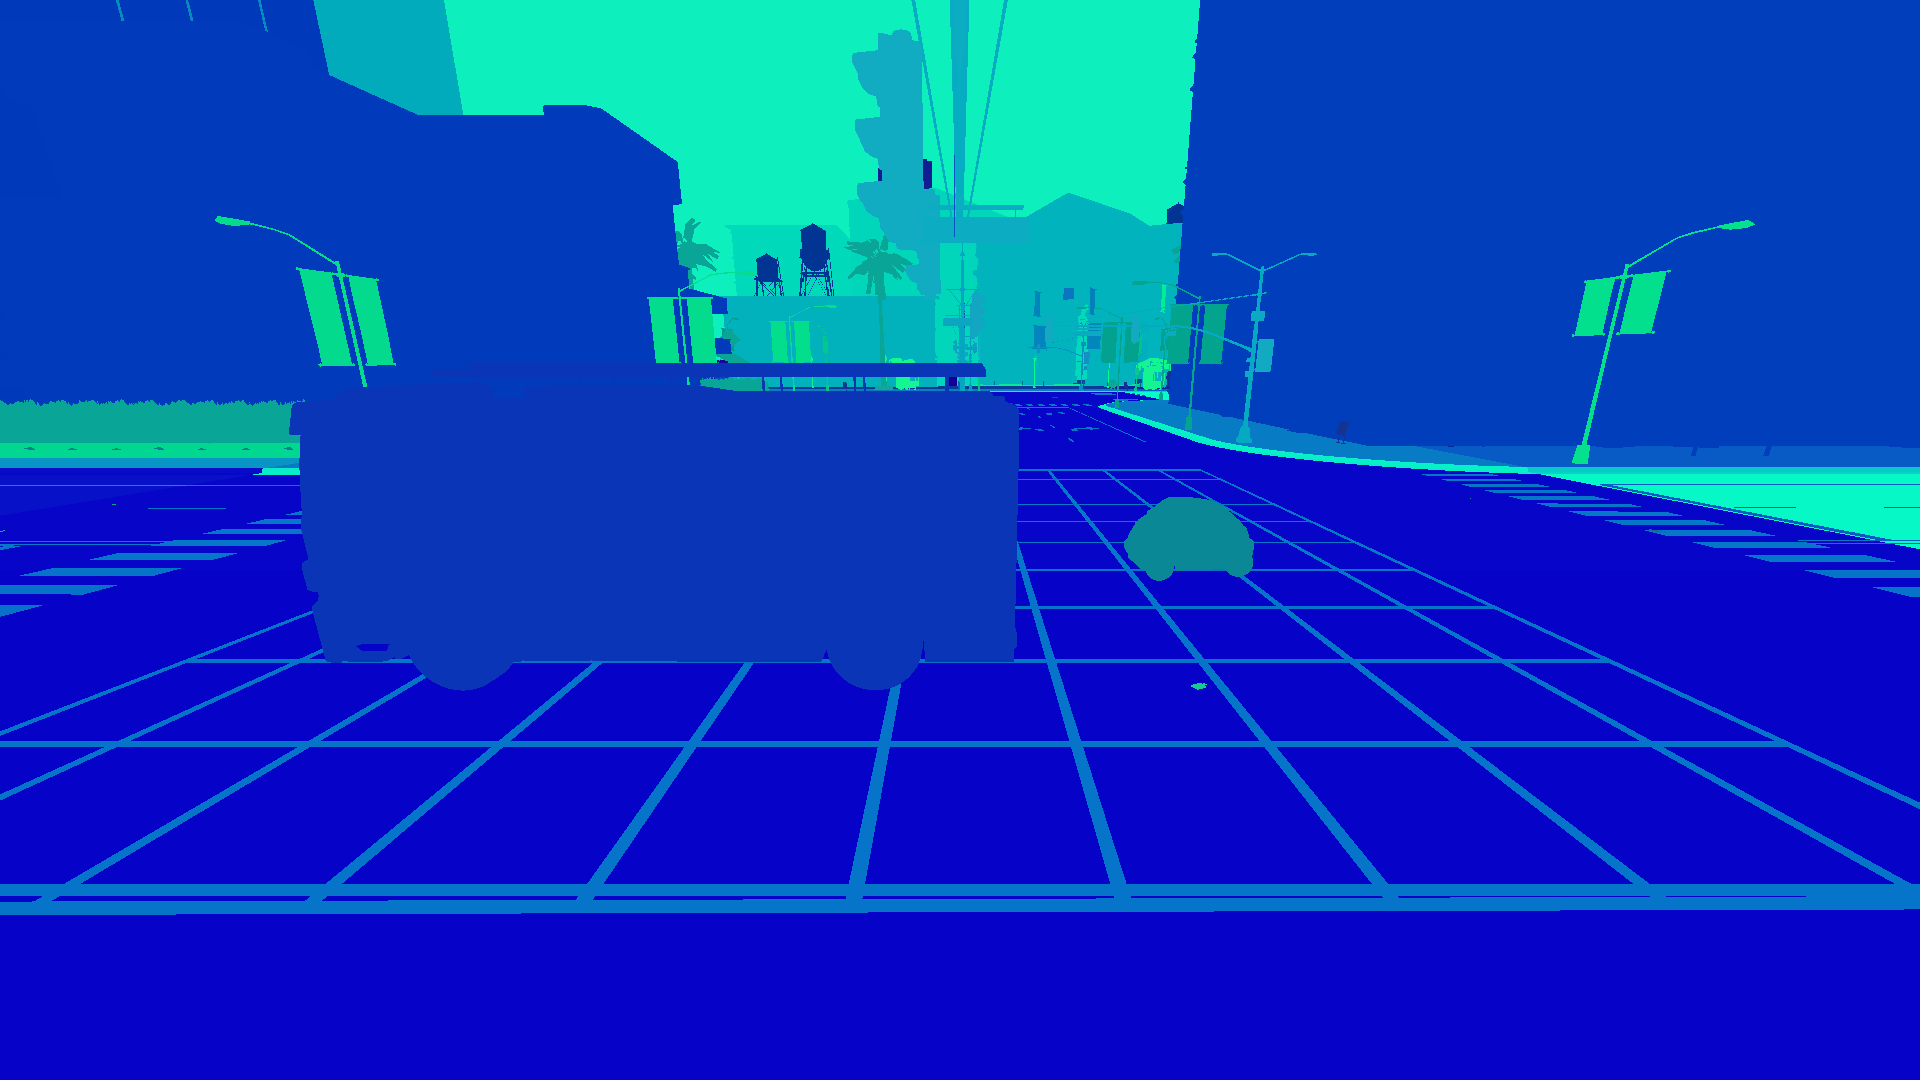
\includegraphics[width=0.5\textwidth]{images/instance_cam.jpg}}
  \caption[CARLA's cameras]{These two images display the difference between the output of the two camera types.} \label{fig:camera_outputs}
\end{figure}
%###################################################################################
%###################### Topic C             ########################################
%###################################################################################
\newpage
\section{Related Work} \label{related_work}
In the latest decades, optimal camera positioning has been constantly researched and investigated in a great number of studies, which have proposed different approaches for solving this problem. The greater part of research papers found deal with sensors placed on vehicles like in \cite{onboard_sensor_placement}, where a framework for an optimal heterogenous sensor placement configurations is presented. Their framework explores the space of a vehicle and generates heterogenous configurations of cameras and other sensors. What is more, the framework is deployed across a 2019 Chevrolet Blazer and a 2016 Chevrolet Camaro to enhance the vehicles' environmental perception with the help of feature performance metrics, i.e., longitudinal position error, object occlusion rate, false positive object detection rate, etc. In the end the effectiveness of their proposal is proven by validating their results with real-drive cycle data. 

Ma et al. present in \cite{surveillance_related_work} five placement strategies based on vehicle traffic for surveillance cameras so that they reach an adequate area coverage. The focus in their work is on reducing the costs accumulated when more cameras as necessary are used. They represent a town as a rigid grid of equal square blocks to achieve map-independence and to have an applicable strategy for each location. Afterwards, they observe different metrics(e.g., how many vehicles pass through a block, how many of them were unique, what time each car has spent in a camera's field of view) and formulate their strategies as maximisation problems. Using greedy algorithm to solve them and real-world data to apply them, they manage to show that their placement strategies could facilitate traffic surveillance in different aspects. 

In a similar work from Gonzalez-Barbosa et al. \cite{total_coverage_optimum}, an Occupancy Grid Map is used as a workspace to determine an optimum for camera placement configuration so that a total coverage is achieved. They implement a binary integer programming algorithm, which is applied to simulations for directional and omnidirectional cameras. Furthermore, sensors are fixed and have predefined constraints in the face of their parameters, i.e., field of view and focal length. The environment also contains some obstacles and occlusions for more realistic experiments. As a result of their experiments, a minimum of both types of cameras is proposed to be effective for providing sufficient coverage of the range of interest. However, the efficiency of omnidirectional cameras is limited to detecting only scene changes, whereas the directional can identify objects because of better resolution.

Another approach for finding an optimal position of roadside cameras is offered by Du et al. in  \cite{occlusion_degree_model}. Unlike the previous papers, which does not take three-dimensional reconstruction into account, here the main point examined is the 3D occlusion, which happens when a large vehicle decreases the range of view of a sensor and covers other traffic participants. It introduces an occlusion degree model (ODM), which measures the occlusion between the occluding vehicle and the occluded one. Furthermore, in their strategy they find the blind zone produced by the occluding vehicle, and after a vehicle enters it the 3D world points are transformed into a 2D image plane points in order to calculate the degree of occlusion. This work conducts its experiments in both simulated and real-world environment by placing their sensors next to the road and considering side factors like traffic density and percentage of trucks, which can influence their performance.

In this thesis, after considering the aforementioned approaches, we decided to use a slightly changed version of the ODM approach in combination with \myworries{ADD HERE SOMETHING} metrics and thus suggest optimal camera positions for an enhanced mobility. 
